\chapter{Desarrollo}
\label{chap:Desarrollo}

\section{1º Iteración: Diseño de la interfaz.}

Lo primero es tener claro cuál sería el diseño más correcto de la interfaz para que así fuera intuitivo 
y fácil de utilizar para el usuario. Contamos con que este vaya ser la persona más alejada de la tecnología posible 
y por tanto la interfaz sea intuitiva y fácil de utilizar. Se propusieron 3 opciones para realizar el diseño:

\subsection{1º Opción}

En esta primera opción, se propuso una tabla donde el usuario indica en cada columna el nombre de datos que quiere 
y mediante un formulario con una ayuda de un LLM recupera los datos del histórico de la empresa.

\begin{figure}[hp!]
    \centering
    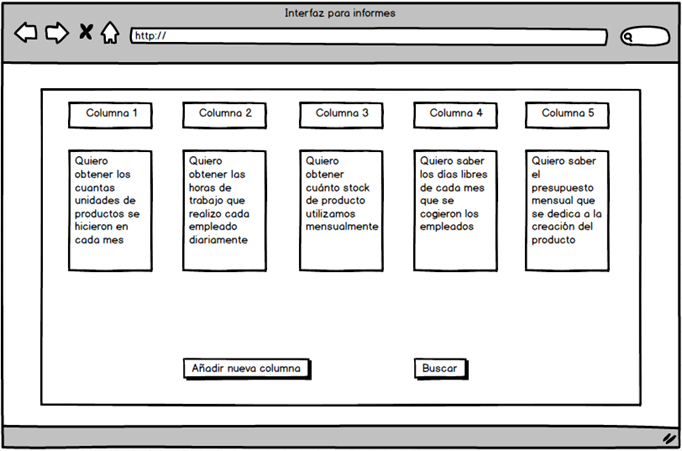
\includegraphics[width=0.75\textwidth]{imaxes/iteracion1.1.png}
    \caption{Primera opción: Tabla con datos para recuperar}
    \label{fig:iteracion1.1}
\end{figure}

El usuario podría introducir las columnas que quisiera e indicaría el nombre del dato que va a recuperar mediante el nombre de la columna. 
Con la ayuda de un formulario donde indicamos los datos que queremos recuperar y procesando esta información mediante un LLM, 
se recuperan estos datos del histórico.

\begin{figure}[hp!]
    \centering
    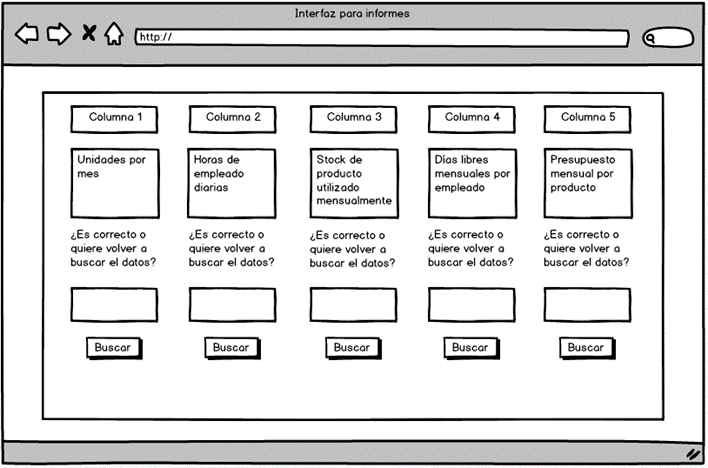
\includegraphics[width=0.75\textwidth]{imaxes/iteracion1.2.png}
    \caption{Primera opción: Tabla con datos recuperados y/o posibles modificaciones}
    \label{fig:iteracion1.2}
\end{figure}

Después de hacer la búsqueda con la ayuda del LLM, se mostrarán los datos que se recuperan de cada columna y tendrá la opción de editar 
alguno de estos datos sino es el que le interesa al usuario
  
Es una solución que permite guiar al usuario paso a paso para seleccionar los datos que quiere en su informe, 
pero tiene un gran problema, y es que, si añadimos muchas columnas, la interfaz se volverá muy compleja, ya que habría 
demasiada información y podría volverse muy confuso.

\subsection{2º Opción}

Esta segunda solución se basaría en un selector con los datos que el usuario quiera ver, los ira seleccionado e ira avanzando progresivamente 
con más selectores hasta tener el dato concreto.

Primero de todo, el usuario selecciona los datos sobre las tablas que le interesa.

\begin{figure}[hp!]
    \centering
    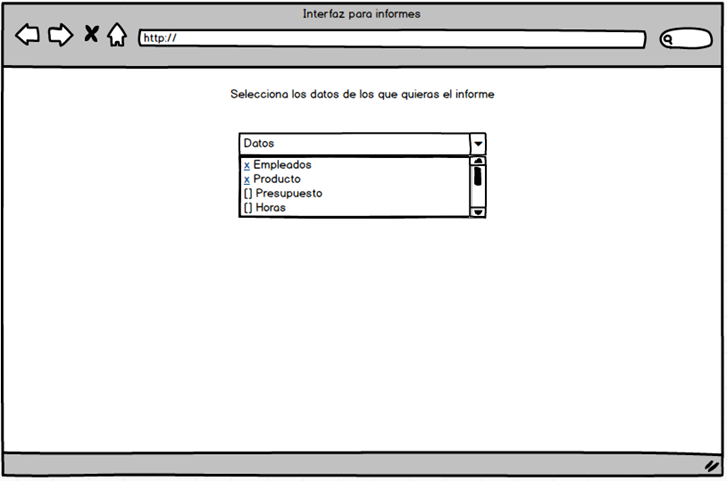
\includegraphics[width=0.75\textwidth]{imaxes/iteracion1.3.png}
    \caption{Segunda opción: Selector con primeras opciones}
    \label{fig:iteracion1.3}
\end{figure}

Después, se irán mostrando las distintas opciones de cada dato seleccionado e se ira avanzando progresivamente mediante selectores.

\begin{figure}[hp!]
    \centering
    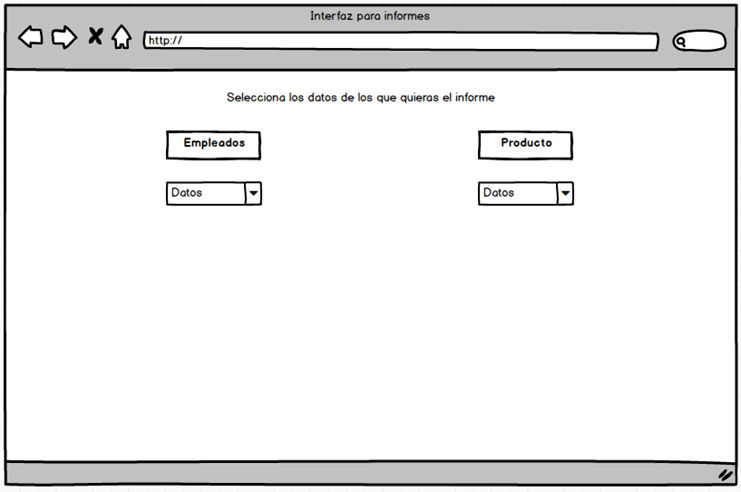
\includegraphics[width=0.75\textwidth]{imaxes/iteracion1.4.png}
    \caption{Segunda opción: Selector las siguientes opciones para acotar nuestro dato}
    \label{fig:iteracion1.4}
\end{figure}

En esta solución, los usuarios pueden ir seleccionando de manera progresiva lo que quieren en su informe, lo que puede ser bastante 
intuitivo para obtener los datos que queremos finalmente, pero tiene el mismo problema que la anterior, al seleccionar muchos datos, 
la interfaz se puede volver bastante engorrosa. También limita a la hora de crear informes complejos, ya que se necesitan muchos pasos 
para crearlos y puede ser una gran pérdida de tiempo para el cliente.

\subsection{3º Opción}

La tercera solución es un pront donde el usuario interactuara con un LLM viendo en un json o una tabla los datos que van ofreciendo y 
seleccionando los datos que más nos interesen mediante inputs.

\begin{figure}[hp!]
    \centering
    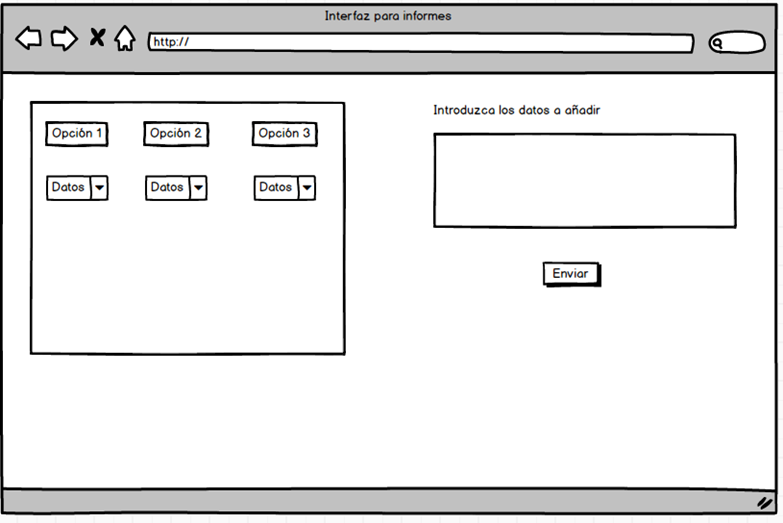
\includegraphics[width=0.75\textwidth]{imaxes/iteracion1.5.png}
    \caption{Tercera opción: Prompt con datos a añadir}
    \label{fig:iteracion1.5}
\end{figure}

El usuario introducirá los datos que le interese en el input y se irán mostrando las distintas opciones de datos 
para los elementos del informe generar.

Esta es una opción bastante buena para la generación de informes complejos, ya que con la ayuda del LLM puede ayudar a 
buscar lo que se necesita de forma correcto, pero esto se puede convertir en una contra también, ya que en el caso contrario 
podría ser que el LLM no entienda claramente lo que se quiere buscar y esto puede ser un problema para un usuario no familiarizado con la interfaz.

\subsection{Conclusión}

De estas 3 opciones, después de estudiar sus pros y contras, se concluyo que la mejor opción sería una mezcla de las 3 de esta forma.

Primero, el usuario seleccionará los datos de los que le interese generar el informe sin sus opciones.

\begin{figure}[hp!]
    \centering
    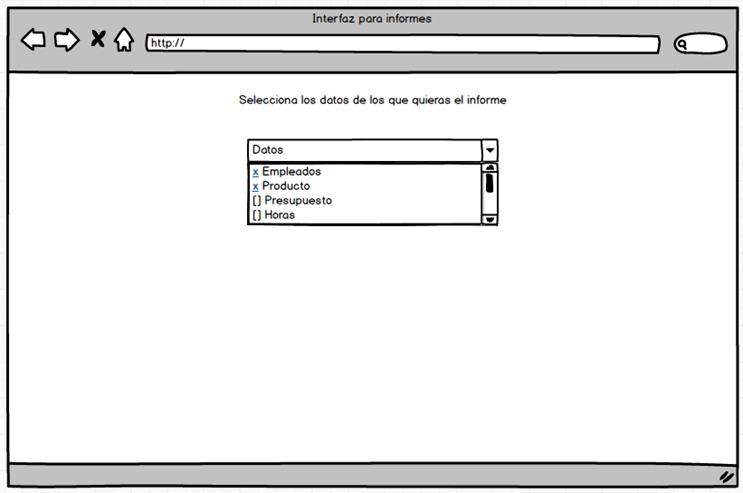
\includegraphics[width=0.75\textwidth]{imaxes/iteracion1.6.png}
    \caption{Conclusión: Seleccionamos los datos que nos interensan}
    \label{fig:iteracion1.6}
\end{figure}

Con los datos seleccionados, se nos mostrará una tablita donde con esos datos y un pront, 
el usuario indicará las opciones que quiere de cada dato recogiendo esa información con un LLM para posteriormente mostrarlo en la tabla.


\begin{figure}[hp!]
    \centering
    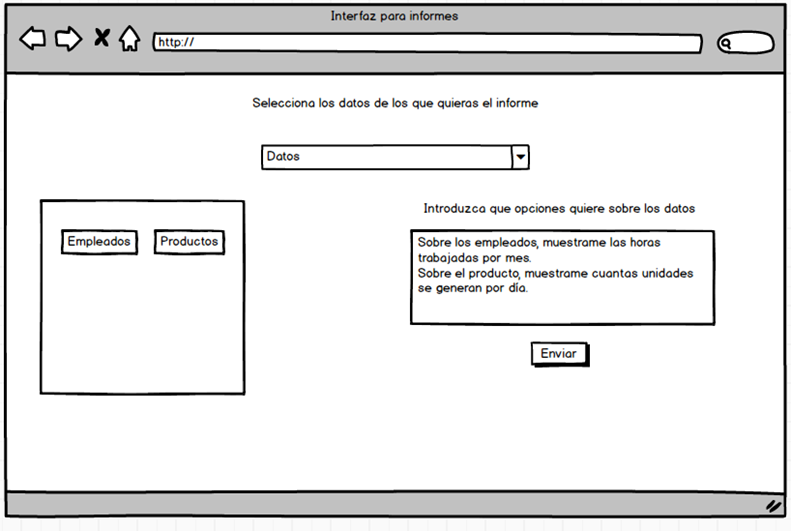
\includegraphics[width=0.75\textwidth]{imaxes/iteracion1.7.png}
    \caption{Conclusión: Tabla con los datos seleccionados y prompt para buscar}
    \label{fig:iteracion1.7}
\end{figure}

Cuando el LLM procesé la información, mostrará un selector desplegable donde se puede seleccionar 
la opción o las opciones que el usuario consideré opinión según lo introducido en el pront y su criterio.

\begin{figure}[hp!]
    \centering
    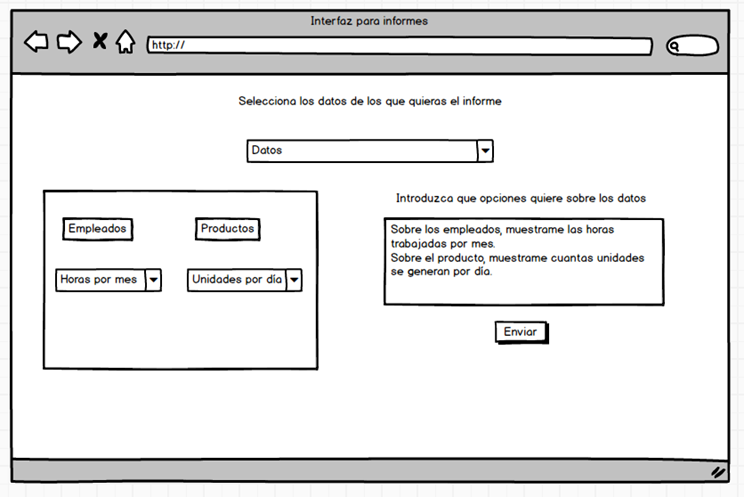
\includegraphics[width=0.75\textwidth]{imaxes/iteracion1.8.png}
    \caption{Conclusión: Tabla con los datos seleccionados y las opciones buscadas anteriormente}
    \label{fig:iteracion1.8}
\end{figure}
  
Esta es la mejor opción mezclando las 3 anteriores, ya que el usuario puede comenzar 
con una serie de columnas claras e ir modificándolas o no según su criterio. Con la ayuda del LLM, 
este nos muestra las opciones más acordes a nuestra búsqueda y ayudando así a no tener que navegar mediante selectores, 
lo cuál es mucho más engorroso para un usuario sin experiencia.
  
\section{2º Iteración: Nueva propuesta de diseño de la interfaz.}

Una vez comentandas las ideas anteriores junta UX, y tras refinarlas, se llego a una conclusión conjunta para como 
se quiere que sea esta interfaz.

En esta nueva pantalla, se nos mostrará diferentes opciones para configurar nuestro informe. 
Se podrá seleccionar la periodicidad con la que se generé (la idea de esta interfaz es que se generé cada x tiempo el informe una vez configurado), 
pudiendo seleccionar las unidades de tiempo y el período en el que se van a generar. 
Podemos ir añadiendo las columnas que creamos oportunas que aparezcan en él y en ellas indicar tanto el nombre como el dato que queremos buscar. 

\begin{figure}[hp!]
    \centering
    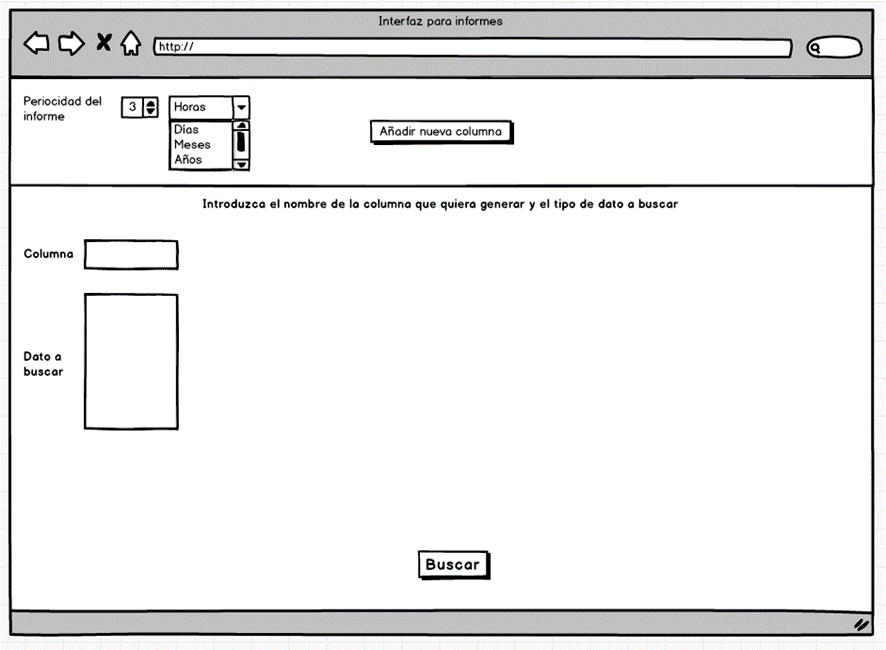
\includegraphics[width=0.75\textwidth]{imaxes/iteracion2.1.png}
    \caption{2º Iteración: Nueva interfaz}
    \label{fig:iteracion2.1}
\end{figure}

Una vez que el usuario introduzca la información que quiera, con la ayuda de un LLM, buscará está en nuestro histórico, 
para así mostrarle posteriormente los datos que busca al usuario.

\begin{figure}[hp!]
    \centering
    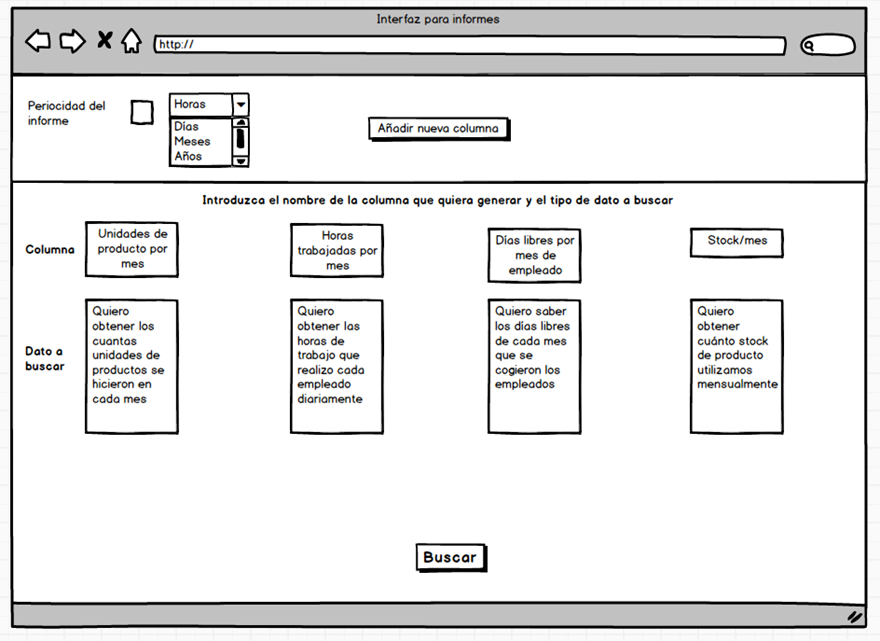
\includegraphics[width=0.75\textwidth]{imaxes/iteracion2.2.png}
    \caption{2º Iteración: Introducir columnas y datos para la busqueda}
    \label{fig:iteracion2.2}
\end{figure}

Si alguno de los datos que aparecen no nos encaja con lo que buscamos, podremos seleccionar mediante un desplegable la columna 
del informe que queremos cambiar y con la ayuda de un prompt, introduciremos los cambios que consideraremos oportunos.

Tendremos también una serie de palabras clave sugeridas para que así esta sea más fácil y nos facilite a la hora de generar el informe.

\begin{figure}[hp!]
    \centering
    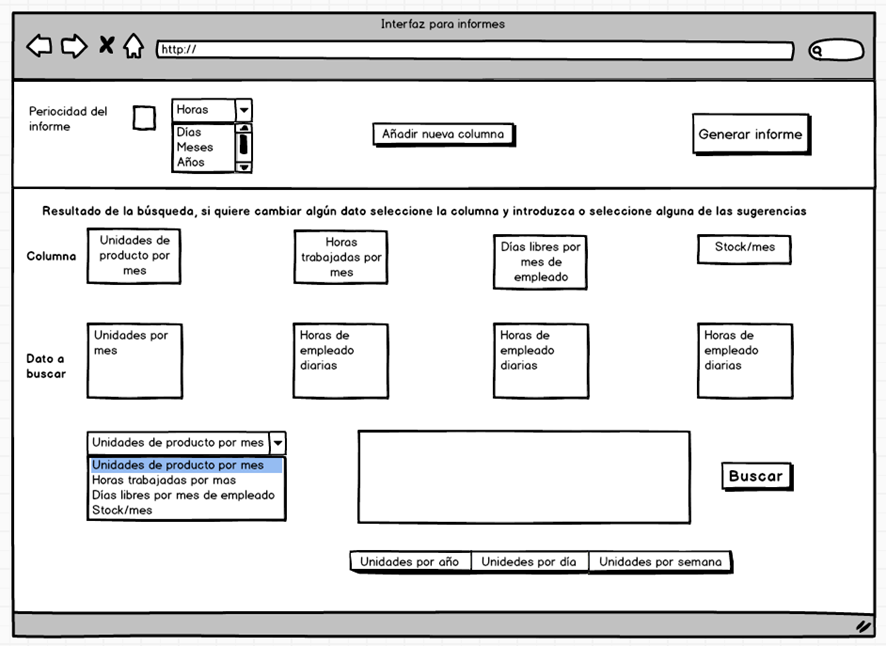
\includegraphics[width=0.75\textwidth]{imaxes/iteracion2.3.png}
    \caption{2º Iteración: Resultados de la búsqueda}
    \label{fig:iteracion2.3}
\end{figure}

\section{3º Iteración: Consolidación de la nueva propuesta.}

Se volvió a comentar la nueva propuesta con UX y se tomaron algunas decisiones de diseño para la interfaz. 
Primero de todo y más importante, habría que definir la finalidad de ese informe y esto se haría a través del título.

Se añadirá un título que describirá el propósito del informe. Para que sea más fácil para el usuario la configuración de este, 
se mostrará una serie de ejemplos donde el usuario podrá ver los diferentes pasos que debe seguir para generar el informe.

\begin{figure}[hp!]
    \centering
    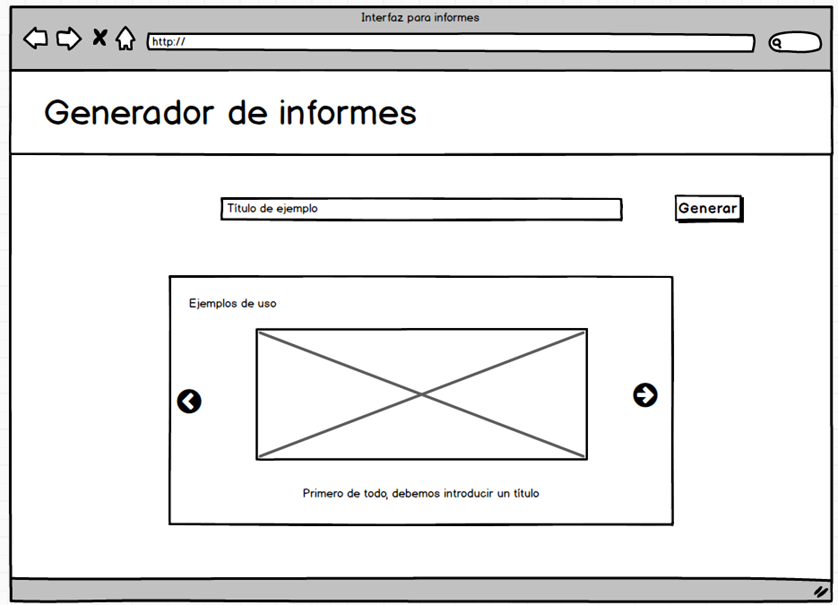
\includegraphics[width=0.75\textwidth]{imaxes/iteracion3.1.png}
    \caption{3º Iteración: Pantalla principal}
    \label{fig:iteracion3.1}
\end{figure}

Una vez añadido el título, se debe configurar el informe. Para esto, se seleccionara la periodicidad con la que se genera 
y el nombre de la columna más el dato que quiera añadir a su informe, como se comento en un principio. 
Si necesita añadir más datos a su informe, añadira una nueva columna a la tabla.

\begin{figure}[hp!]
    \centering
    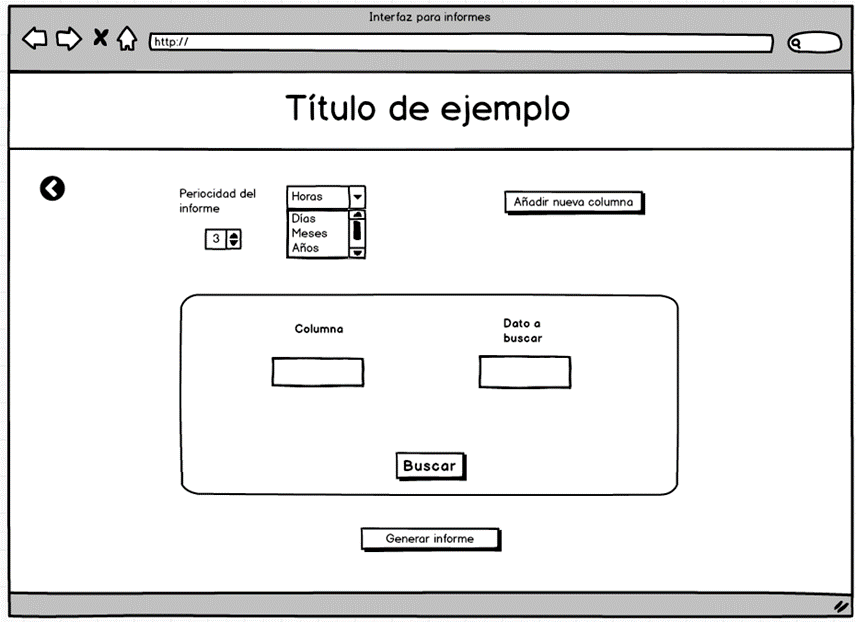
\includegraphics[width=0.75\textwidth]{imaxes/iteracion3.2.png}
    \caption{3º Iteración: Configurador de informe}
    \label{fig:iteracion3.2}
\end{figure}

En este caso, se añadieron 2 columnas con los datos oportunos para buscarlos.

\begin{figure}[hp!]
    \centering
    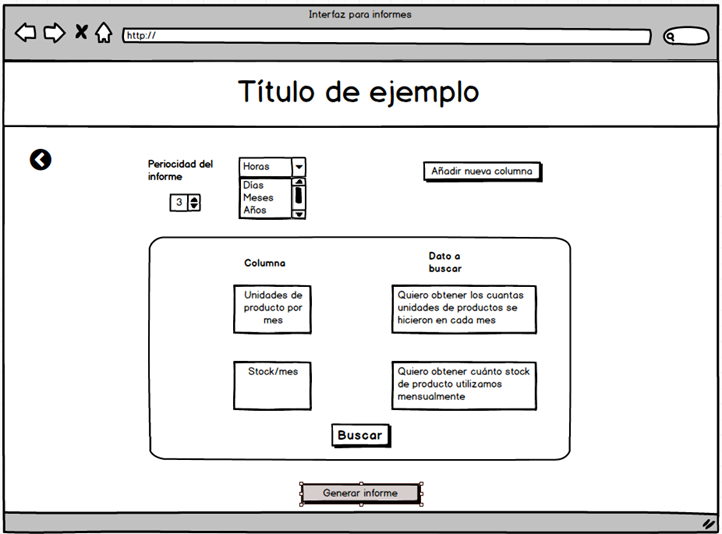
\includegraphics[width=0.75\textwidth]{imaxes/iteracion3.3.png}
    \caption{3º Iteración: Introducir datos de ejemplo para buscar}
    \label{fig:iteracion3.3}
\end{figure}

A la hora de buscar estos datos, se mostrarían las opciones que al LLM le pareció más oportuno según los 
datos registrados en el histórico. Podrá seleccionar las distintas columnas del informe y mediante un prompt 
con algunas opciones sugeridas, poder refinar su búsqueda para que se muestre el dato de forma correcta

\begin{figure}[hp!]
    \centering
    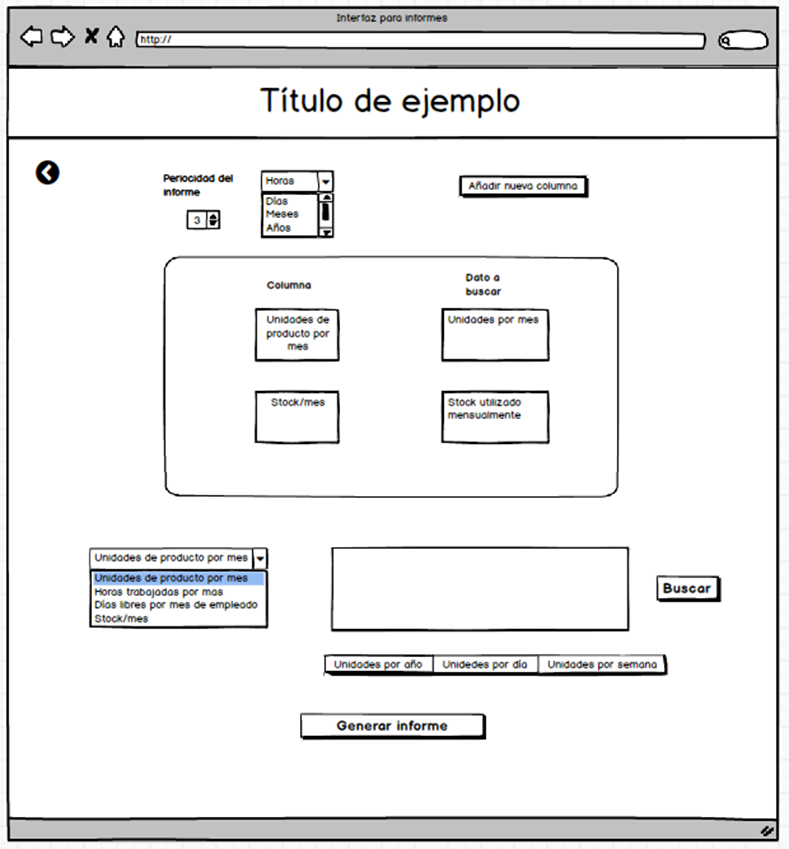
\includegraphics[width=0.75\textwidth]{imaxes/iteracion3.4.png}
    \caption{3º Iteración: Resultados de la búsqueda}
    \label{fig:iteracion3.4}
\end{figure}

Si el usuario tiene claro que los datos son correctos, puede generar el informe, 
que quedara configurado para generarse periódicamente según el tiempo que le haya indicado.